\documentclass[conference]{IEEEtran}

\usepackage{cite}
\usepackage{amsmath,amssymb}
\usepackage{algorithm}
\usepackage{algorithmic}
\usepackage{booktabs}
\usepackage{graphicx}
\usepackage{url}
\usepackage{xurl}
\usepackage{array}
\usepackage{multirow}
\usepackage{balance}
\usepackage[hidelinks,breaklinks=true]{hyperref}

\graphicspath{{figures/}}
\setlength{\textfloatsep}{5pt}
\setlength{\floatsep}{4pt}
\setlength{\abovedisplayskip}{4pt}
\setlength{\belowdisplayskip}{4pt}
\setlength{\abovecaptionskip}{2pt}
\setlength{\belowcaptionskip}{0pt}

\begin{document}

\title{RACS: Reliability-Aware Congestion-Stressed Scheduling for Earth Observation in LEO Satellite Networks}

\author{
\IEEEauthorblockN{K. Deepak Chowdary, Suvadip Hazra, and Rajendra Hegadi}
\IEEEauthorblockA{Department of Computer Science and Engineering, IIIT Dharwad, India\\
Email: deepak.24phdcs02@iiitdwd.ac.in, suvadip@iiitdwd.ac.in, rajendra.h@iiitdwd.ac.in}
}

\maketitle

\begin{abstract}
Low-Earth-orbit (LEO) satellite constellations can support time-sensitive Earth observation (EO) services, but task scheduling becomes difficult when observation opportunities, satellite-to-ground downlinks, inter-satellite links, deadlines, priorities, and link congestion interact. This paper studies reliability-aware EO task scheduling using a congestion-stressed LEO satellite dataset containing normal and congested instances with up to 40 satellites, 100 meta-tasks, 252 atomic observation tasks, 48,662 observation windows, and 1,042 satellite-to-ground windows. We formulate each EO meta-task as a deadline-constrained group of atomic observations that must be observed and downlinked before its deadline. We then propose a Reliability-Aware Congestion-Stressed scheduler (RACS) that jointly considers meta-task priority, deadline urgency, completion delay, downlink congestion, reliability margin, and uncertainty. Unlike single-satellite policies, RACS can split atomic observations across feasible visible satellites, use multiple downlink windows, and use relay-assisted downlink when direct satellite-to-ground delivery is infeasible. Across base scenarios, RACS improves average completion rate from 0.900 to 0.958 in normal cases and from 0.713 to 0.743 in congested cases compared with reliability-only scheduling. Under combined deadline, bandwidth, and data-volume stress, RACS improves completion rate from 0.626 to 0.806 and reduces deadline miss rate from 0.374 to 0.194. Results show that congestion-aware multi-satellite scheduling delivers the highest value when EO workloads face tight deadlines and limited downlink capacity.
\end{abstract}

\begin{IEEEkeywords}
LEO satellite networks, Earth observation, task scheduling, congestion awareness, reliability, inter-satellite links, downlink scheduling
\end{IEEEkeywords}

\section{Introduction}
LEO satellite constellations are increasingly used for Earth observation, remote sensing, disaster monitoring, and low-latency space information services. EO task scheduling in such networks is difficult because a request is not completed when an image is captured; the generated data must also be delivered to a ground station before the deadline. Therefore, a feasible schedule must jointly handle observation windows, generated data volume, satellite-to-ground (S2G) downlink capacity, inter-satellite link (ISL) opportunities, meta-task priorities, and deadlines.

This work complements two earlier parts of our LEO reliability research. The first studied risk-aware visibility-window reliability using survival analysis \cite{deepak_visibility}. The second studied disagreement-aware service path selection under structural shift in open LEO measurements \cite{deepak_disagreement}. The present paper is technically distinct: it studies EO scheduling decisions, where the question is which meta-tasks should be observed, through which satellites, and through which delivery opportunities under congestion.

\emph{Research gap:} most classical satellite task-scheduling work focuses on observation-window assignment, priority maximization, or visibility-aware association. In congestion-stressed LEO networks, this is insufficient. A satellite may be visible for observation but unable to downlink the produced data before the deadline. Similarly, choosing the earliest or highest-priority task may overload scarce S2G windows and reduce the number of completed EO products. \emph{The key distinction of this paper is full-chain service completion under congestion: observation feasibility, S2G capacity, one-hop ISL fallback, multi-satellite atomic-task splitting, and deadline reliability are evaluated together before a meta-task is accepted.} This paper does not claim a globally optimal scheduler; it proposes a reproducible online heuristic for this stricter scheduling model.

The main contributions are:
\begin{itemize}
\item We formulate EO task scheduling as a reliability-aware, congestion-stressed LEO scheduling problem involving atomic observations, S2G downlink capacity, ISL relay opportunities, deadlines, and meta-task priorities.
\item We propose RACS, a lightweight heuristic scheduler that combines reliability margin, congestion ratio, urgency, priority, delay, multi-satellite atomic-task splitting, split downlink, and one-hop relay fallback.
\item We evaluate seven scheduling policies on normal, congested, and controlled stress scenarios using dataset instances from 5 to 40 satellites, and report ablation comparisons, bootstrap confidence intervals, runtime, fairness, and relay/downlink diagnostics.
\item We show that the largest benefit appears under combined congestion stress. RACS improves completion by 18 percentage points over reliability-only scheduling while reducing deadline misses and downlink congestion.
\end{itemize}

\section{Related Work}
\subsection{LEO Network Reliability and Measurements}
LEO networks experience fast topology changes, intermittent visibility, and limited contact duration. Prior work has studied LEO topology dynamics, routing, and emulation platforms such as Hypatia and StarryNet \cite{bhattacherjee2018space,kassing2020hypatia,lai2023starrynet}. Measurement-driven studies show that real LEO systems exhibit short-term variability, outages, and location-dependent performance \cite{mohan2024starlink,zhao2024lens}. Our earlier work on survival-based visibility-window modeling focused on estimating usable service time and drop risk \cite{deepak_visibility}, while our path-selection work used predictor disagreement as a risk signal under structural shift \cite{deepak_disagreement}. The present work applies the same reliability-aware perspective to EO task scheduling with explicit downlink congestion.

\subsection{EO Task Scheduling}
Satellite EO scheduling has been widely studied as a constrained optimization problem involving observation windows, priorities, deadlines, and resource conflicts \cite{wang2019survey,chen2020satellite}. Recent EO networking work has also studied downlink-latency reduction through semantic communication and distributed satellite edge processing \cite{hassan2024semantic,mercado2024vessel}. Exact optimization can be useful for small instances, while genetic, rule-based, and learning-based heuristics are commonly used when the search space grows. Online or large-scale LEO scheduling often requires fast heuristics because task arrivals, contact windows, and network load change quickly. Many studies emphasize observation assignment, semantic reduction, or processing placement; in contrast, this paper focuses on deadline-constrained completion of EO meta-tasks through observation and S2G/ISL delivery.

\subsection{Congestion and Multi-Hop Space Networking}
Downlink bottlenecks and ISL-assisted routing are central to modern LEO systems \cite{kodheli2021survey,lu2024opensn}. Congestion-aware resource allocation is especially important when multiple meta-tasks compete for the same S2G windows. The dataset used here explicitly includes observation, S2G, and ISL windows, enabling evaluation of whether a scheduler benefits from multi-satellite assignment and relay-assisted delivery rather than treating each meta-task as a single-satellite decision.

\subsection{Positioning Against Prior Work}
Compared with visibility-only association, RACS does not accept a meta-task merely because a satellite can observe it; it requires a complete observation-and-delivery chain. Compared with classical EO scheduling, it explicitly scores downlink congestion and delivery uncertainty, not only observation priority and deadline. Compared with generic multi-satellite assignment, it allows atomic observations of the same EO meta-task to be distributed across visible satellites and then delivered through split S2G windows or one-hop relay fallback. Thus, the paper treats S2G/ISL delivery as a first-class scheduling constraint rather than as a post-observation assumption.

\section{System Model and Problem Formulation}
\subsection{Network and Task Model}
Let $\mathcal{S}$ be the set of LEO satellites, $\mathcal{G}$ the ground stations, and $\mathcal{T}$ the set of EO meta-tasks. Each meta-task $i\in\mathcal{T}$ has priority $p_i$, arrival time $a_i$, deadline $d_i$, and a set of atomic observation tasks $\mathcal{A}_i$. Atomic task $j\in\mathcal{A}_i$ has observation duration $\tau_j$ and generated data volume $v_j$.

The dataset provides three window sets: observation windows $\mathcal{W}^{obs}$, S2G downlink windows $\mathcal{W}^{s2g}$, and ISL windows $\mathcal{W}^{isl}$. An observation window indicates that satellite $s$ can observe atomic task $j$ during $[b,e]$. An S2G window indicates that satellite $s$ can downlink to ground station $g$ with bandwidth $B$ during $[b,e]$. The corresponding capacity is
\begin{equation}
C^{s2g}_{w} = \frac{B_w(e_w-b_w)}{8},
\end{equation}
where bandwidth is in Gbps and capacity is measured in GB. A meta-task is completed only if every atomic task is observed after $a_i$ and all generated data are downlinked before $d_i$.

\begin{figure*}[t]
\centering
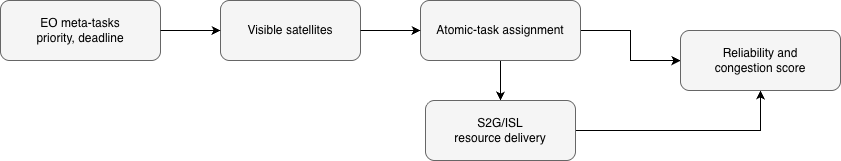
\includegraphics[width=0.98\textwidth]{system_model.png}
\caption{System model for reliability-aware congestion-stressed EO task scheduling. EO meta-tasks are first filtered through visible satellite opportunities, atomic observations are assigned, S2G/ISL delivery resources are checked, and the final reliability--congestion score determines whether resources are reserved.}
\label{fig:system}
\end{figure*}

\subsection{Reliability and Congestion Metrics}
For a candidate plan $q$ of task $i$, let $t^c_i$ be completion time, $V_i=\sum_{j\in\mathcal{A}_i} v_j$ be generated volume, and $C_q$ be reserved downlink capacity. The slack and congestion ratio are
\begin{equation}
L_q=d_i-t^c_i,\qquad \rho_q=\frac{V_i}{\max(C_q,\epsilon)}.
\end{equation}
The reliability score combines deadline margin and downlink capacity margin:
\begin{equation}
R_q=0.55\sigma\left(\frac{L_q}{1800}\right)+0.45\sigma\left(\frac{C_q-V_i}{2}\right),
\end{equation}
where $\sigma(x)=1/(1+e^{-x})$. The uncertainty score is
\begin{equation}
U_q=\min(1,\rho_q)(1-R_q).
\end{equation}
This score is high when a plan is both congested and unreliable.

\subsection{Scheduling Objective}
The scheduler should maximize completed priority-weighted EO work while reducing deadline misses and congestion:
\begin{equation}
\max \sum_{i\in\mathcal{T}} x_i p_i
\end{equation}
subject to observation-window conflicts, S2G capacity, ISL availability, and $t^c_i\leq d_i$ for accepted meta-tasks. Here $x_i=1$ if meta-task $i$ is completed and $0$ otherwise. Because exact global optimization is expensive for online decision-making, this paper evaluates lightweight policies that build feasible schedules sequentially.

\section{Proposed RACS Scheduler}
RACS first orders meta-tasks using deadline tightness, priority, and volume. For each meta-task, it searches all visible satellites for each atomic observation. Unlike a single-satellite policy, RACS may assign different atomic observations of the same meta-task to different satellites. This assumption is operationally meaningful when a meta-task consists of multiple independent image tiles, sensing points, or sub-areas that can be collected separately and fused at the ground segment. It is less appropriate for monolithic observations that require one continuous pass by the same satellite. RACS then attempts direct split downlink. If direct S2G delivery is infeasible, it checks one-hop ISL relay opportunities and downlinks through the relay satellite. Relay is limited to one hop by design to keep online search bounded and reproducible. This is not a claim that deeper relay chains are unimportant in operational networks; it is a scoped design choice for the benchmarked scheduling problem.

For each feasible plan $q$, RACS uses a weighted multi-objective score
\begin{equation}
\begin{split}
S_q ={}& 4.0\frac{p_i}{10}+2.8R_q+1.2H_i+0.4M_q\\
&-2.2\rho_q-1.6U_q-0.15N^{relay}_q-0.15D_q,
\end{split}
\end{equation}
where $H_i$ is urgency, $M_q$ is split-assignment gain, $N^{relay}_q$ is the number of relay uses, and $D_q$ is normalized completion delay. The weights are normalization constants selected to prioritize completion reliability and downlink capacity margin over small delay differences. They are not learned parameters, and the paper does not claim that this weight vector is globally optimal. The main empirical claim is therefore not coefficient optimality; it is that full-chain feasibility expansion through atomic splitting, split downlink, and bounded relay improves completion under congestion stress.

\subsection{Design Rationale}
The score in (6) is designed to avoid a common weakness of priority-only and deadline-only rules: they may select meta-tasks that are attractive locally but consume scarce delivery capacity. The reliability term rewards plans with remaining deadline and downlink-capacity margin. The congestion term penalizes plans that nearly exhaust a selected S2G window. The split-gain term encourages use of multiple satellites only when this increases feasibility, while the relay penalty discourages unnecessary ISL use when direct downlink is already available. Thus, RACS is best understood as a feasibility-first, weighted multi-objective heuristic for complete EO service delivery.

\subsection{Computational Cost}
For a meta-task with $A_i$ atomic observations, $|\mathcal{S}|$ satellites, at most $W^{obs}$ observation windows per atomic task, $W^{s2g}$ downlink windows per satellite, and $W^{isl}$ relay windows, the dominant search cost is approximately
\begin{equation}
O(A_i|\mathcal{S}|W^{obs}+|\mathcal{S}|(W^{s2g}+W^{isl}W^{s2g})).
\end{equation}
This is suitable for online heuristic scheduling because the algorithm checks feasible windows directly and reserves resources greedily. The dominant factor in the evaluated instances is the observation-candidate search over satellites and atomic tasks, followed by S2G/ISL delivery checks. RACS does not solve a global mixed-integer program, so it trades optimality guarantees for low implementation complexity and fast rescheduling.

\begin{algorithm}[t]
\caption{RACS: Reliability-Aware Congestion-Stressed Scheduling}
\label{alg:racs}
\begin{algorithmic}[1]
\REQUIRE Meta-tasks $\mathcal{T}$, observation windows, S2G windows, ISL windows
\STATE Sort meta-tasks by deadline tightness, priority, and data volume
\STATE Initialize satellite resource reservations as empty
\FOR{each meta-task $i$ in sorted order}
    \STATE Generate observation candidates for every atomic task using all visible satellites
    \IF{any atomic task has no feasible observation}
        \STATE reject meta-task $i$
    \ELSE
        \STATE assign atomic tasks to earliest feasible satellites with low resource load
        \STATE compute generated volume per selected satellite
        \STATE find direct split S2G downlink windows before deadline
        \IF{direct downlink is infeasible}
            \STATE search one-hop ISL relay and relay-satellite downlink
        \ENDIF
        \IF{observation and delivery are feasible}
            \STATE compute $R_q$, $\rho_q$, $U_q$, and $S_q$
            \STATE accept meta-task and reserve observation/downlink/relay resources
        \ELSE
            \STATE reject meta-task $i$
        \ENDIF
    \ENDIF
\ENDFOR
\RETURN completed schedule and rejected meta-tasks
\end{algorithmic}
\end{algorithm}

\section{Experimental Setup}
\subsection{Dataset}
We use the congestion-stressed LEO satellite network dataset for EO task scheduling from IEEE DataPort \cite{dataport_eo}. It contains normal and congested instances from 5 to 40 satellites. Table~\ref{tab:dataset} summarizes the instances.

\begin{table}[t]
\caption{Dataset instances used in the evaluation. Each normal/congested entry reports the corresponding pair of instance sizes.}
\label{tab:dataset}
\centering
\scriptsize
\begin{tabular}{lrrrrr}
\toprule
Instance & Sat. & Tasks & Atomic & Obs. win. & S2G win.\\
\midrule
S05 normal/cong. & 5 & 15/5 & 38/14 & 1107/197 & 132/78\\
S10 normal/cong. & 10 & 30/10 & 75/29 & 3594/1069 & 262/151\\
S20 normal/cong. & 20 & 60/30 & 151/92 & 14252/6613 & 525/300\\
S40 normal/cong. & 40 & 100/60 & 252/185 & 48662/28331 & 1042/618\\
Tiny stress test & 5 & 5 & 5 & 38 & 26\\
\bottomrule
\end{tabular}
\end{table}

\subsection{Baselines and Metrics}
We compare seven policies: earliest-deadline-first (EDF), highest-priority-first (HPF), shortest-task-first (STF), congestion-unaware, reliability-only, a single-satellite reliability-congestion policy, and RACS. The metrics are completion rate, normalized priority reward, deadline miss rate, mean congestion ratio, mean reliability score, and Jain fairness over priority-class completion rates \cite{jain1984fairness}.

To test robustness beyond base instances, four controlled stress settings are applied: tight deadlines (deadline factor 0.70), reduced bandwidth (S2G bandwidth factor 0.65), high data volume (volume factor 1.35), and combined stress (deadline factor 0.65, bandwidth factor 0.60, volume factor 1.35).

\subsection{Implementation Notes}
All policies use the same parsed task, observation-window, S2G-window, and ISL-window tables. For non-proposed baselines, a meta-task is scheduled through a single selected satellite and one downlink window. For RACS, atomic observations may be distributed across multiple visible satellites, and the generated volume may be delivered through more than one downlink window. A meta-task is counted as completed only after all atomic observations and all required downlink segments are reserved before the deadline. This strict completion rule avoids overstating performance from observation-only schedules.

\subsection{Statistical and Runtime Evaluation}
Because each dataset instance is deterministic, repeated random trials would not provide independent evidence. Instead, we report instance-level bootstrap confidence intervals over the available instances and use paired tests across matched instances. Runtime is measured by repeatedly evaluating all instances and reporting mean milliseconds per instance on the same machine.

We also implemented a restricted candidate-plan MILP check for the 5-satellite instances. It optimizes selection over pre-generated feasible candidate plans, but it is not a full exact solver because it does not enumerate all possible observation/downlink timing combinations. Therefore, it is reported only as a sanity check and must not be interpreted as an optimal benchmark or optimality-gap certificate.

\section{Results and Discussion}
\subsection{Base Normal and Congested Scenarios}
Table~\ref{tab:base_results} shows average results by scenario group. In normal instances, RACS increases completion rate from 0.900 for reliability-only scheduling to 0.958, while reducing deadline miss rate from 0.100 to 0.042. In congested instances, the margin is smaller but consistent: completion improves from 0.713 to 0.743, and mean congestion ratio decreases from 0.323 to 0.272. This indicates that RACS accepts more meta-tasks while using less congested delivery plans.

\begin{table}[t]
\caption{Average base-scenario results by policy group. Comp. is the completed meta-task fraction, Reward is normalized completed priority, Miss is the deadline-miss fraction, and Cong. is mean downlink congestion ratio.}
\label{tab:base_results}
\centering
\scriptsize
\begin{tabular}{llrrrr}
\toprule
Case & Policy & Comp. & Reward & Miss & Cong.\\
\midrule
\multirow{4}{*}{Normal}
& EDF & 0.864 & 0.874 & 0.136 & 0.157\\
& HPF & 0.898 & 0.911 & 0.103 & 0.155\\
& Rel.-only & 0.900 & 0.914 & 0.100 & 0.159\\
& RACS & \textbf{0.958} & \textbf{0.960} & \textbf{0.042} & \textbf{0.113}\\
\midrule
\multirow{4}{*}{Cong.}
& EDF & 0.710 & 0.734 & 0.290 & 0.327\\
& HPF & 0.713 & 0.738 & 0.287 & 0.328\\
& Rel.-only & 0.713 & 0.738 & 0.287 & 0.323\\
& RACS & \textbf{0.743} & \textbf{0.752} & \textbf{0.257} & \textbf{0.272}\\
\bottomrule
\end{tabular}
\end{table}

\begin{figure}[t]
\centering
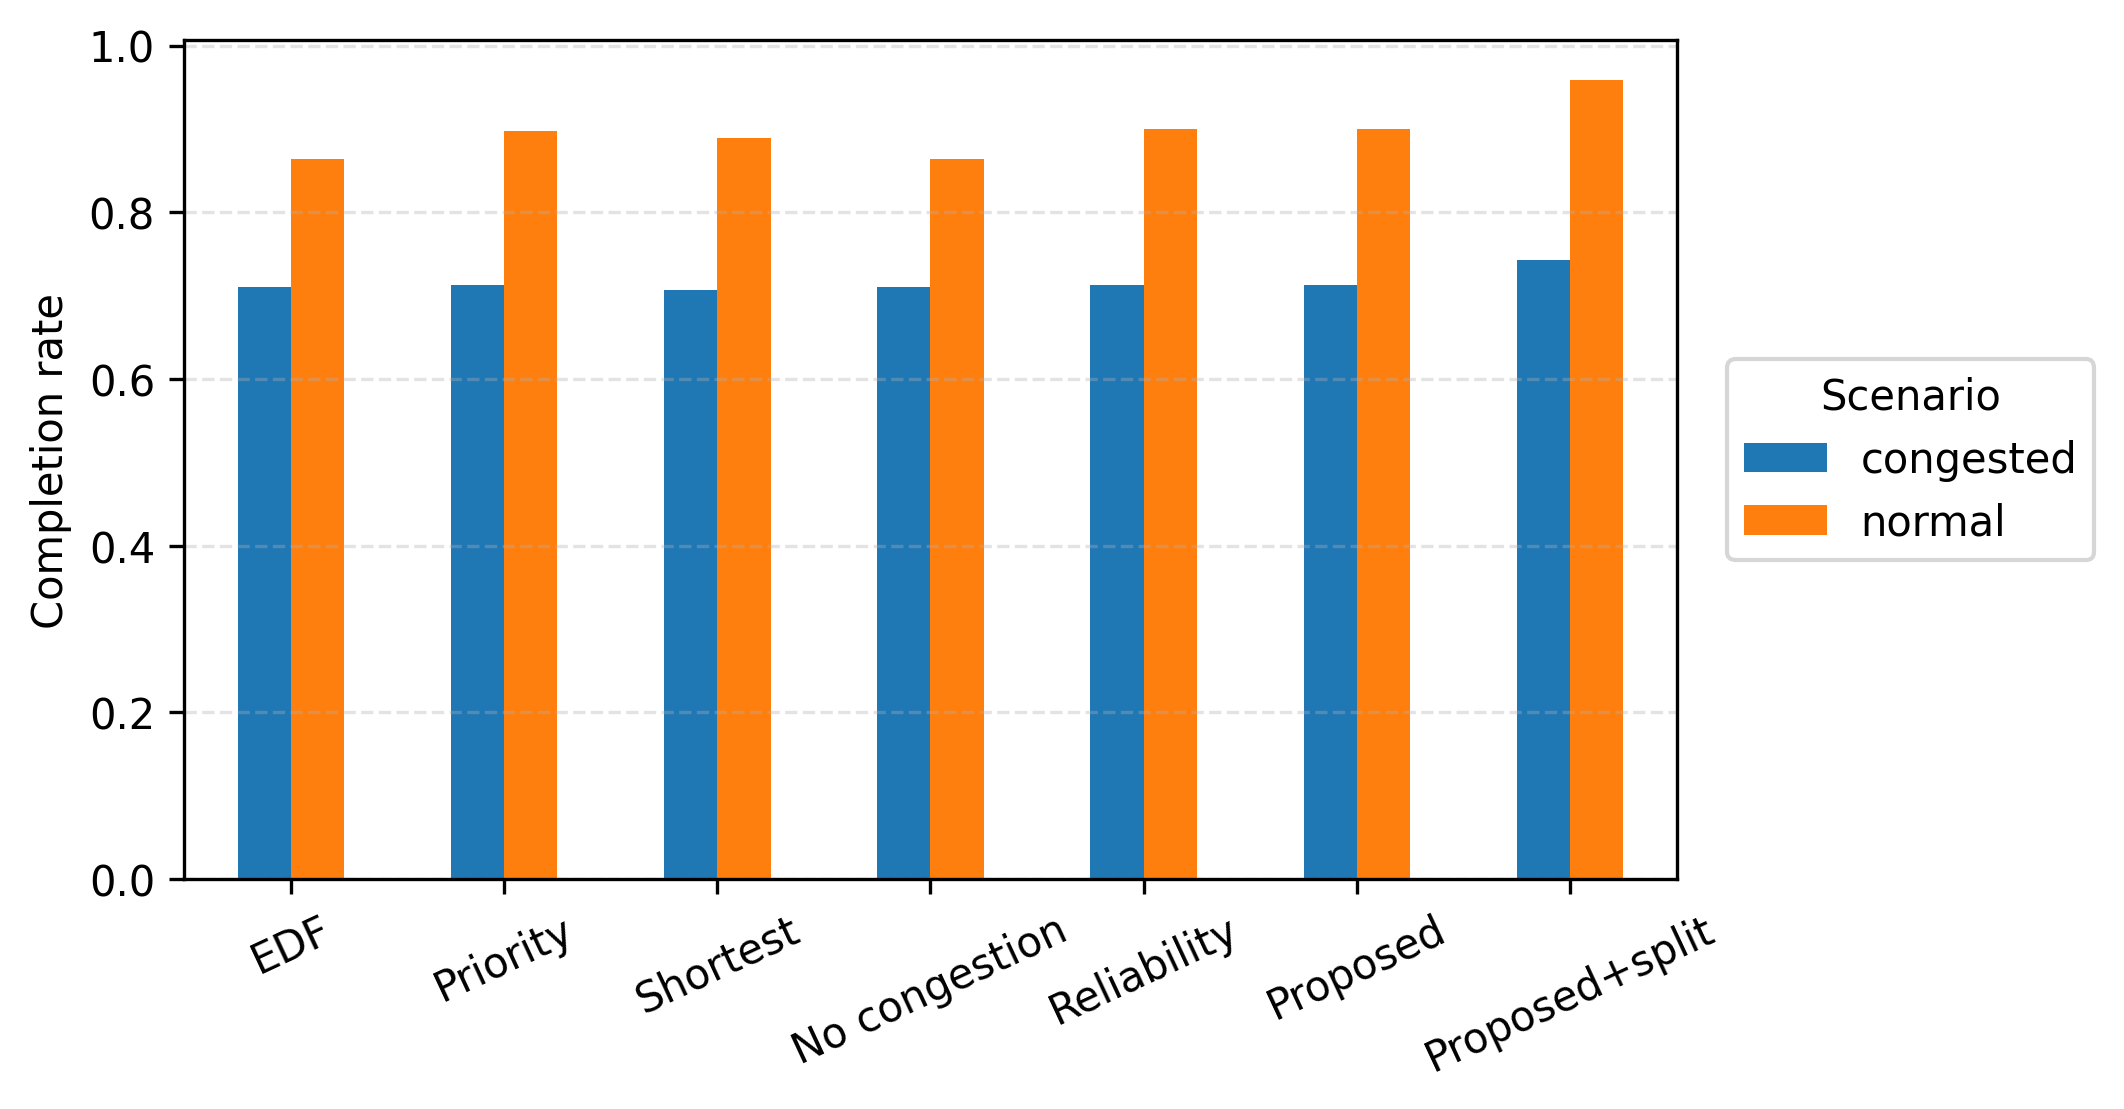
\includegraphics[width=\columnwidth]{completion_rate_by_policy.png}
\caption{Base-scenario completion rate. RACS completes the largest fraction of EO meta-tasks in both normal and congested groups.}
\label{fig:completion}
\end{figure}

\subsection{Stress Scenarios}
The benefit of RACS is clearer under controlled stress. Table~\ref{tab:stress_results} reports representative stress results. Under combined stress, RACS improves completion rate from 0.626 to 0.806 compared with reliability-only scheduling and reduces deadline miss rate from 0.374 to 0.194. The gain comes from using feasible visible satellites, splitting downlink across multiple windows, and using relay fallback when direct delivery is insufficient.

\begin{table}[t]
\caption{Controlled-stress results for reliability-only scheduling and RACS. RACS has the largest advantage when deadline, bandwidth, and data-volume stress are combined.}
\label{tab:stress_results}
\centering
\scriptsize
\begin{tabular}{llrrrr}
\toprule
Stress & Policy & Comp. & Reward & Miss & Cong.\\
\midrule
\multirow{2}{*}{Tight deadline}
& Rel.-only & 0.776 & 0.793 & 0.224 & 0.249\\
& RACS & \textbf{0.830} & \textbf{0.836} & \textbf{0.170} & \textbf{0.203}\\
\midrule
\multirow{2}{*}{Reduced BW}
& Rel.-only & 0.791 & 0.808 & 0.209 & 0.361\\
& RACS & \textbf{0.837} & \textbf{0.844} & \textbf{0.163} & \textbf{0.302}\\
\midrule
\multirow{2}{*}{High volume}
& Rel.-only & 0.794 & 0.813 & 0.206 & 0.327\\
& RACS & \textbf{0.839} & \textbf{0.845} & \textbf{0.161} & \textbf{0.268}\\
\midrule
\multirow{2}{*}{Combined}
& Rel.-only & 0.626 & 0.606 & 0.374 & 0.425\\
& RACS & \textbf{0.806} & \textbf{0.814} & \textbf{0.194} & \textbf{0.369}\\
\bottomrule
\end{tabular}
\end{table}

\begin{figure}[t]
\centering
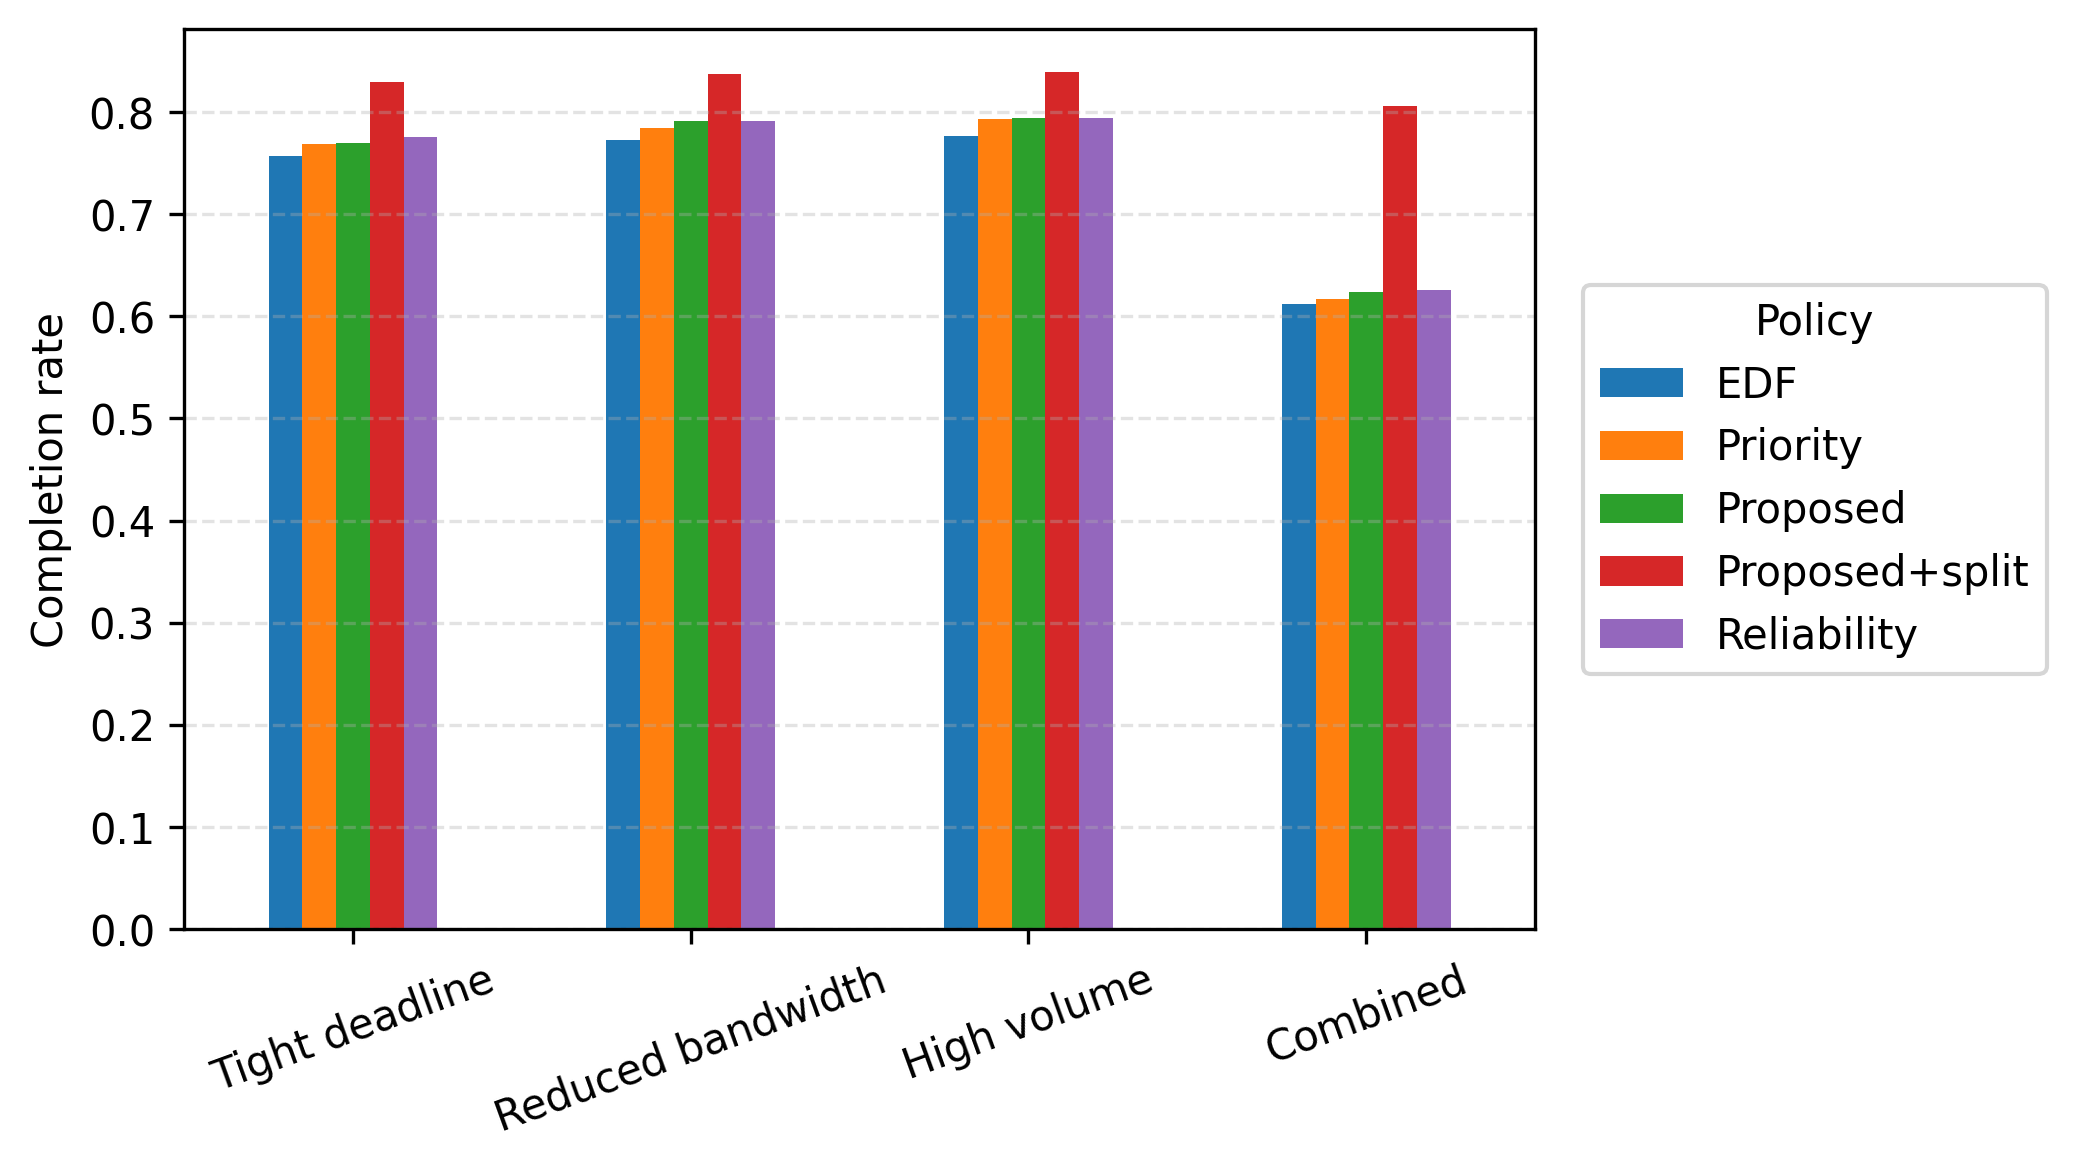
\includegraphics[width=\columnwidth]{stress_completion_rate.png}
\caption{Completion rate under controlled stress. The largest separation occurs under combined deadline, bandwidth, and data-volume stress.}
\label{fig:stress_completion}
\end{figure}

\subsection{Ablation, Confidence, and Runtime}
Table~\ref{tab:ablation} summarizes the effect of adding congestion awareness and then full multi-satellite split/relay capability. In combined stress, reliability-only scheduling completes 0.626 of meta-tasks. Adding only single-satellite congestion awareness reduces congestion but does not improve completion because it still uses one selected satellite and one downlink window. Full RACS improves completion to 0.806 and reduces deadline miss rate to 0.194. The 95\% bootstrap confidence interval for the completion improvement over reliability-only is $[0.119,0.237]$.

\begin{table}[t]
\caption{Combined-stress ablation and runtime. Single-satellite congestion awareness reduces congestion but does not increase completion; full RACS improves completion through multi-satellite assignment and split/relay delivery.}
\label{tab:ablation}
\centering
\scriptsize
\begin{tabular}{lrrrr}
\toprule
Policy & Comp. & Miss & Cong. & ms/inst.\\
\midrule
Rel.-only & 0.626 & 0.374 & 0.425 & 13.30\\
Single-sat. rel.-cong. & 0.624 & 0.376 & 0.404 & 12.93\\
RACS & \textbf{0.806} & \textbf{0.194} & \textbf{0.369} & \textbf{9.86}\\
\bottomrule
\end{tabular}
\end{table}

On the three 5-satellite instances, the restricted candidate-plan MILP check completes 0.667 of meta-tasks on average, while RACS completes 0.689. This does not prove optimality, but it shows that RACS is competitive with an offline candidate-selection check on the smallest cases.

Fig.~\ref{fig:score_sensitivity} reports a score-guided sensitivity check under combined stress. Perturbing the congestion, uncertainty, and relay penalties by 0.5x and 1.5x keeps completion in a narrow range from 0.785 to 0.791. This supports the interpretation that the main gain is driven by full-chain feasibility expansion rather than by a fragile single coefficient choice.

\begin{figure}[t]
\centering
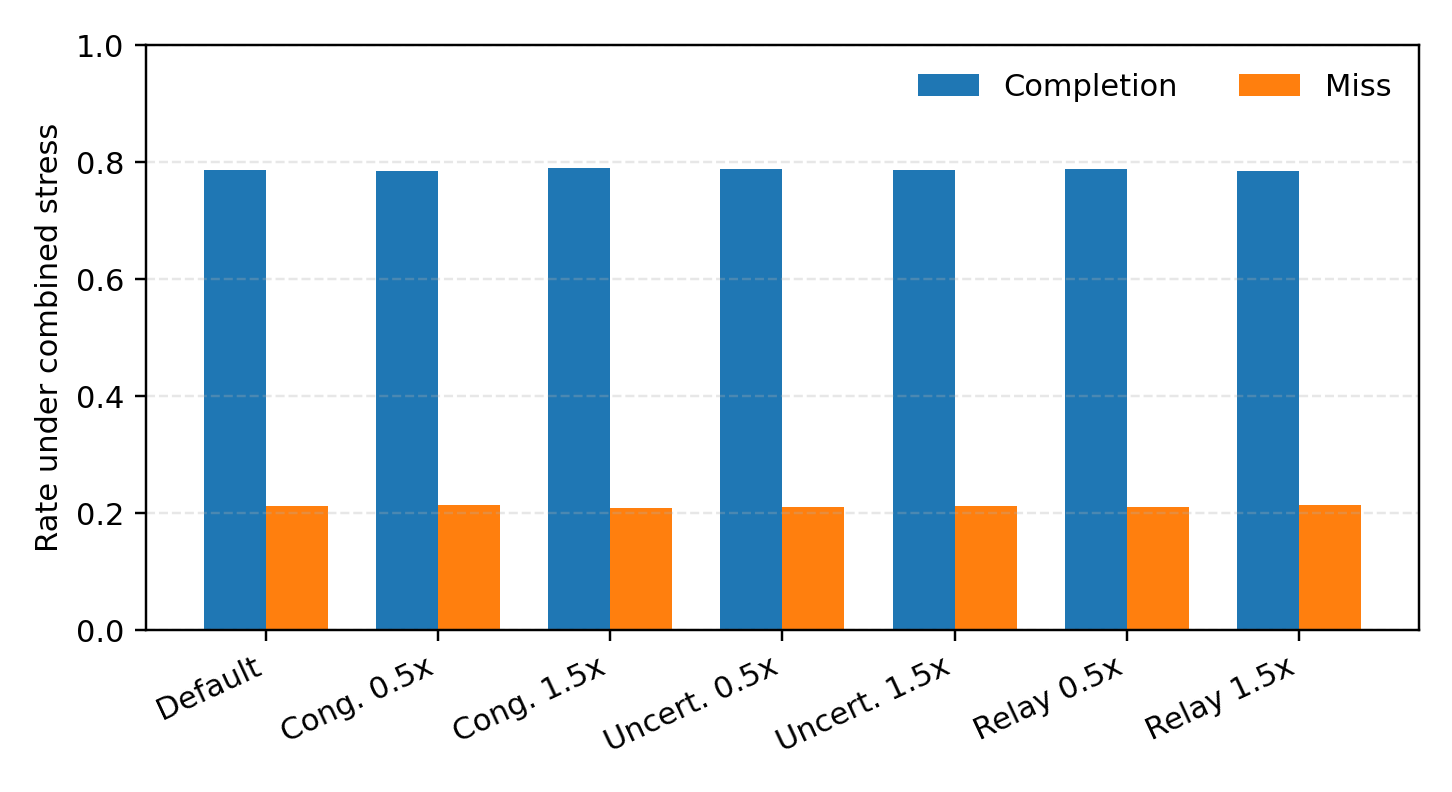
\includegraphics[width=\columnwidth]{score_weight_sensitivity.png}
\caption{Score-weight sensitivity under combined stress. Congestion, uncertainty, and relay penalties in Eq. (6) are perturbed by 0.5x and 1.5x; completion and miss rates remain stable.}
\label{fig:score_sensitivity}
\end{figure}

Table~\ref{tab:statistical} reports the instance-level statistical evidence for RACS over reliability-only scheduling. The base cases have positive bootstrap intervals but limited paired-test power because they contain only four normal and five congested instances. The combined-stress result is stronger, with a paired Wilcoxon completion-rate $p$-value of 0.00195.

\begin{table}[t]
\caption{RACS improvement over reliability-only scheduling. Confidence intervals are instance-level bootstrap intervals for metric differences.}
\label{tab:statistical}
\centering
\scriptsize
\begin{tabular}{lrrrr}
\toprule
Scenario & $\Delta$Comp. CI & $\Delta$Miss CI & $\Delta$Cong. CI & $p$\\
\midrule
Normal & [0.017,0.092] & [-0.092,-0.017] & [-0.051,-0.041] & 0.125\\
Cong. & [0.003,0.067] & [-0.067,-0.003] & [-0.085,-0.016] & 0.125\\
Combined & [0.119,0.237] & [-0.237,-0.119] & [-0.089,-0.018] & 0.00195\\
\bottomrule
\end{tabular}
\end{table}

Fig.~\ref{fig:runtime_scaling} reports runtime scaling by constellation size on normal instances. Runtime grows with satellites, tasks, and window count, but remains below 45 ms for the largest 40-satellite, 100-task instance. This supports the use of RACS as a lightweight online heuristic rather than as an offline global optimizer.

\begin{figure}[t]
\centering
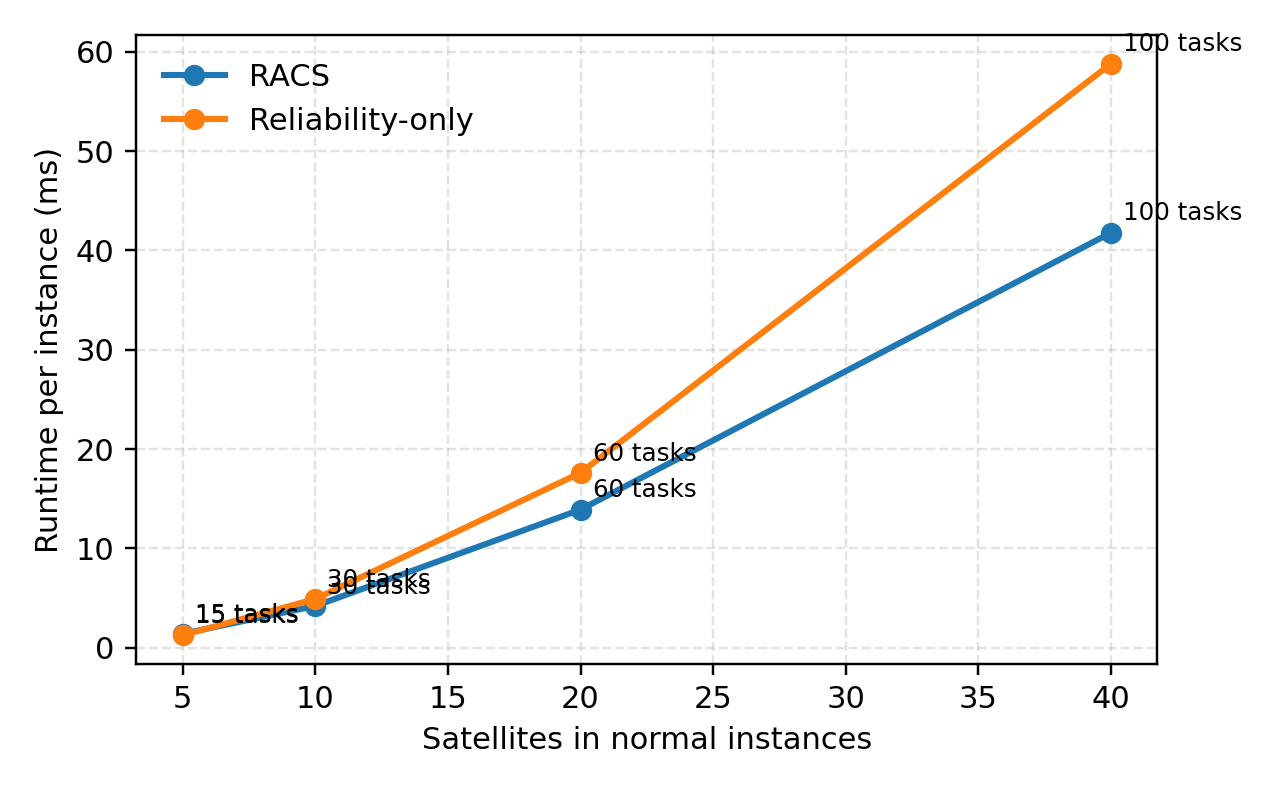
\includegraphics[width=\columnwidth]{runtime_scaling_by_satellites.png}
\caption{Runtime scaling on normal instances. Labels show the number of EO meta-tasks in each instance; RACS remains below 45 ms on the 40-satellite, 100-task case.}
\label{fig:runtime_scaling}
\end{figure}

\subsection{Fairness, Relay Use, and Mechanism}
Table~\ref{tab:diagnostics} explains the mechanism behind the gains. Reliability-only and single-satellite reliability-congestion policies examine many visible satellites, but complete each accepted meta-task through one satellite and one downlink window. RACS expands the feasible action space by considering more atomic-level satellite choices and by using an average of 1.595 downlink windows per completed meta-task. Relay use is low, which indicates that ISL is used as a fallback rather than as the default path.

\begin{table}[t]
\caption{Completed-task assignment diagnostics. RACS increases the feasible atomic-level assignment space and uses more downlink windows while keeping relay use occasional.}
\label{tab:diagnostics}
\centering
\scriptsize
\begin{tabular}{lrrrr}
\toprule
Policy & Visible & Feasible & Relay & DL win.\\
\midrule
Rel.-only & 28.90 & 12.08 & 0.000 & 1.000\\
Single-sat. rel.-cong. & 28.90 & 11.94 & 0.000 & 1.000\\
RACS & \textbf{28.46} & \textbf{60.10} & 0.066 & \textbf{1.595}\\
\bottomrule
\end{tabular}
\end{table}

Fairness also improves under stress. In combined stress, Jain priority-class fairness increases from 0.803 for reliability-only scheduling to 0.877 for RACS. This is relevant for EO service because a scheduler that completes only high-volume or easy low-priority jobs can starve other mission classes. RACS does not improve fairness by sacrificing urgent service: high-priority completion increases from 0.593 to 0.863, while normalized priority reward increases from 0.606 to 0.814.

\subsection{Interpretation}
The base congested results show moderate gains because many meta-tasks remain feasible for several policies. The stress experiments reveal the value of the proposed design. When bandwidth is reduced, data volume increases, or deadlines tighten, single-satellite and single-window policies lose feasible plans quickly. RACS remains stronger because it can use multiple satellites, reserve multiple downlink windows, and use relay-assisted delivery.

\subsection{Limitations and Threats to Validity}
The main limitation is that RACS is still a greedy online heuristic, not a globally optimal mixed-integer optimization solver. Therefore, the results should be interpreted as evidence that reliability and congestion awareness are useful for lightweight online scheduling, not as proof of optimality. The score weights in (6) are heuristic; the sensitivity check in Fig.~\ref{fig:score_sensitivity} is encouraging but not exhaustive. The dataset is synthetic/benchmark-oriented rather than a complete operational constellation trace, so absolute completion rates should not be interpreted as operator-level performance. The congestion model, ISL availability, and S2G bandwidth assumptions may differ from deployed constellations. Future work should add a full exact comparator on small instances, extend relay routing beyond one hop, include onboard storage explicitly, and evaluate dynamic task arrivals with weather- and ground-station-specific disruptions.

\section{Conclusion}
This paper presented RACS, a reliability-aware congestion-stressed EO task scheduler for LEO satellite networks. The proposed scheduler jointly considers meta-task priority, urgency, delay, reliability margin, congestion, uncertainty, multi-satellite assignment, split downlink, and relay fallback. On benchmarked congestion-stressed LEO EO instances, RACS improves completion rate, priority reward, deadline miss rate, and congestion ratio over EDF, HPF, reliability-only, and single-satellite reliability-congestion baselines. The largest gains appear under combined stress, where RACS improves completion rate by 18 percentage points over reliability-only scheduling. These results support reliability-aware decision-making for benchmarked LEO EO scheduling, but they should not be interpreted as direct operator-wide deployment validation.

\balance
\begin{thebibliography}{99}
\bibitem{deepak_visibility}
K. Deepak Chowdary, S. Hazra, and R. Hegadi, ``Risk-aware evaluation of LEO satellite visibility windows using survival analysis,'' manuscript, 2026.

\bibitem{deepak_disagreement}
K. Deepak Chowdary, S. Hazra, and R. Hegadi, ``Disagreement-aware predictive path selection for open LEO measurements under structural shift,'' manuscript, 2026.

\bibitem{dataport_eo}
IEEE DataPort, ``Congestion-stressed LEO satellite network dataset for Earth observation task scheduling and routing,'' dataset, 2026. [Online]. Available: \url{https://ieee-dataport.org/documents/congestion-stressed-leo-satellite-network-dataset-earth-observation-task-scheduling-and}

\bibitem{bhattacherjee2018space}
D. Bhattacherjee, W. Aqeel, I. N. Bozkurt, A. Aguirre, B. Chandrasekaran, P. B. Godfrey, G. Laughlin, B. Maggs, and A. Singla, ``Gearing up for the 21st century space race,'' in \emph{Proc. ACM HotNets}, 2018, pp. 113--119.

\bibitem{kassing2020hypatia}
S. Kassing, D. Bhattacherjee, A. B. A. Godfrey, and A. Singla, ``Exploring the internet from space with Hypatia,'' in \emph{Proc. ACM Internet Measurement Conference}, 2020, pp. 214--229.

\bibitem{lai2023starrynet}
Z. Lai, H. Li, Y. Deng, Q. Wu, J. Liu, Y. Li, J. Liu, L. Liu, and K. Xu, ``StarryNet: Empowering researchers to evaluate futuristic integrated space and terrestrial networks,'' in \emph{Proc. USENIX NSDI}, 2023, pp. 1309--1324.

\bibitem{mohan2024starlink}
N. Mohan, L. Ravindranath, and J. Ott, ``A multifaceted look at Starlink performance,'' in \emph{Proc. ACM Web Conference}, 2024, pp. 2723--2734.

\bibitem{zhao2024lens}
B. Zhao and J. Pan, ``LENS: A LEO satellite network measurement dataset,'' in \emph{Proc. ACM MMSys}, 2024, pp. 1--6.

\bibitem{wang2019survey}
P. Wang, G. Reinelt, P. Gao, and Y. Tan, ``A model, a heuristic and a decision support system to solve the scheduling problem of an Earth observing satellite constellation,'' \emph{Computers \& Industrial Engineering}, vol. 61, no. 2, pp. 322--335, 2011.

\bibitem{chen2020satellite}
H. Chen, J. Li, and X. Wang, ``A survey of satellite observation scheduling models and algorithms,'' \emph{Journal of Systems Engineering and Electronics}, vol. 31, no. 5, pp. 1013--1027, 2020.

\bibitem{hassan2024semantic}
S. S. Hassan, L. X. Nguyen, Y. K. Tun, Z. Han, and C. S. Hong, ``Semantic enabled 6G LEO satellite communication for Earth observation: A resource-constrained network optimization,'' arXiv:2408.03959, 2024.

\bibitem{mercado2024vessel}
A. M. Mercado-Martinez, B. Soret, and A. Jurado-Navas, ``Goal-oriented vessel detection with distributed computing in a LEO satellite constellation,'' arXiv:2410.07431, 2024.

\bibitem{kodheli2021survey}
O. Kodheli \emph{et al.}, ``Satellite communications in the new space era: A survey and future challenges,'' \emph{IEEE Communications Surveys \& Tutorials}, vol. 23, no. 1, pp. 70--109, 2021.

\bibitem{lu2024opensn}
Y. Lu, Y. Wang, J. Liu, and X. Zhang, ``OpenSN: An open-source integrated satellite-terrestrial network simulator,'' \emph{IEEE Network}, vol. 38, no. 2, pp. 166--174, 2024.

\bibitem{jain1984fairness}
R. Jain, D.-M. Chiu, and W. Hawe, ``A quantitative measure of fairness and discrimination for resource allocation in shared computer systems,'' DEC Research Report TR-301, 1984.

\end{thebibliography}

\end{document}
